\section{Results}
\subsection{Research question 1}
For research question 1 the results are 2-dimensional plotted using a line diagram.

\subsubsection{Utility}
\begin{figure}[!htb]
  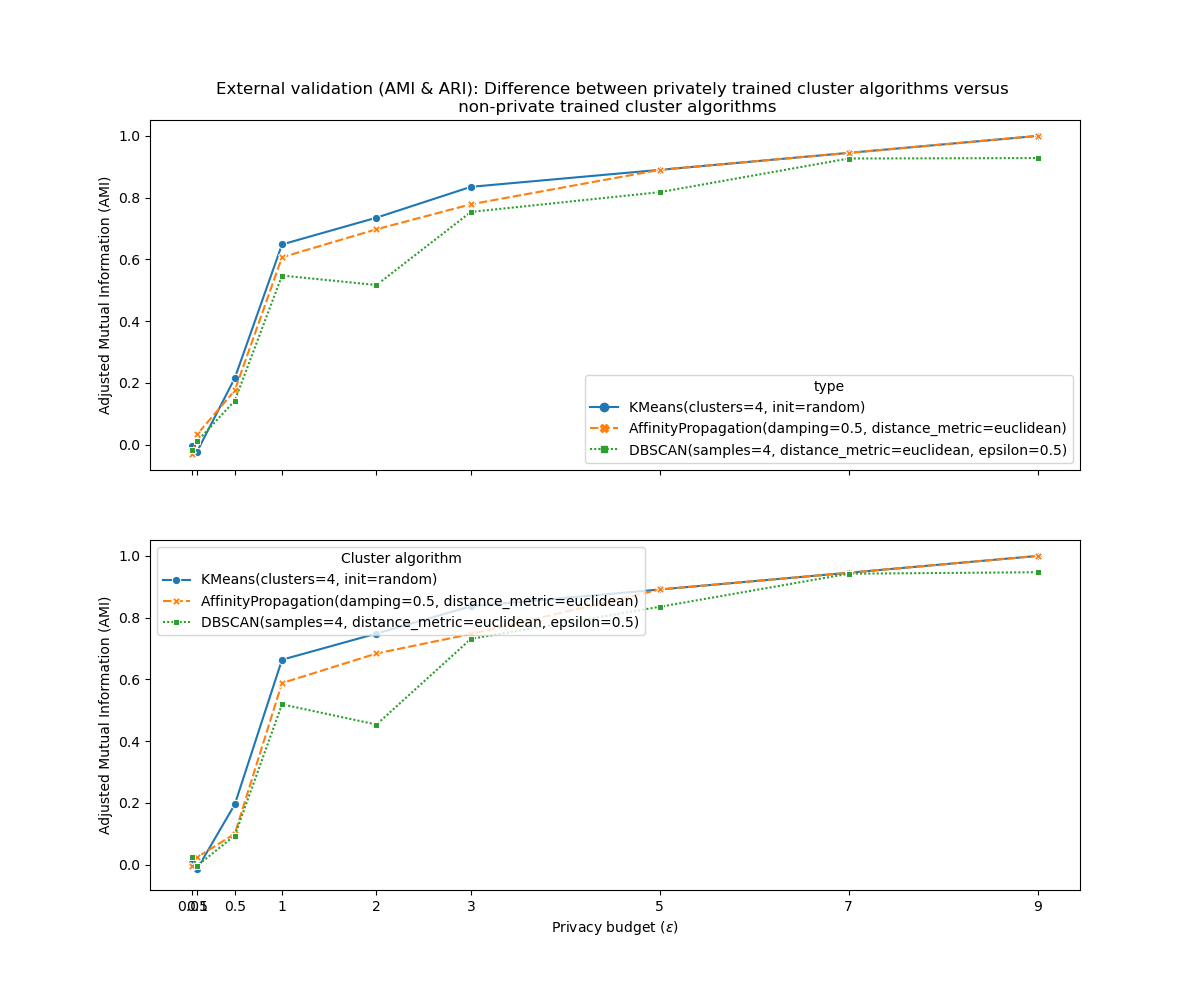
\includegraphics[width=1\linewidth]{Results/rq1/ami-and-ari.png}
  \caption{ARI and AMI evaluation for cluster algorithms 2D-Laplace for a dataset with shape (50, 2)}
\end{figure}
\begin{figure}[!htb]
  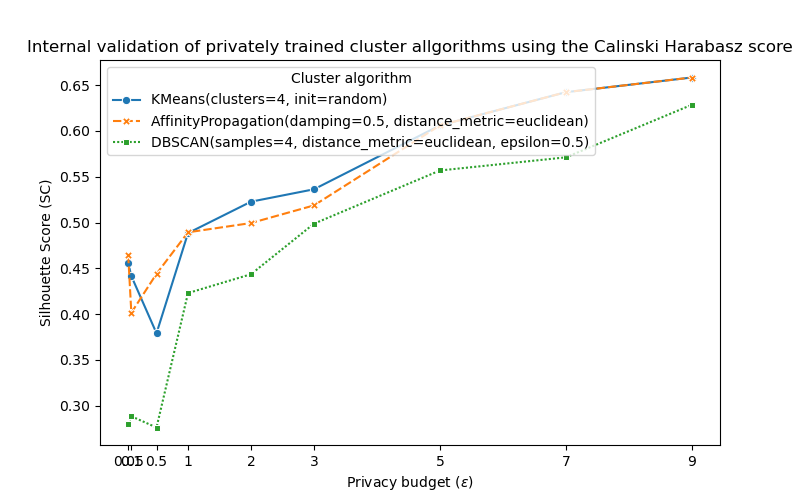
\includegraphics[width=1\linewidth]{Results/rq1/sc.png}
  \caption{SH and CH for cluster algorithms trained with 2D-Laplace for a dataset with shape (50, 2)}
\end{figure}
\newpage
\subsubsection{Privacy}

\begin{figure}[!htb]
  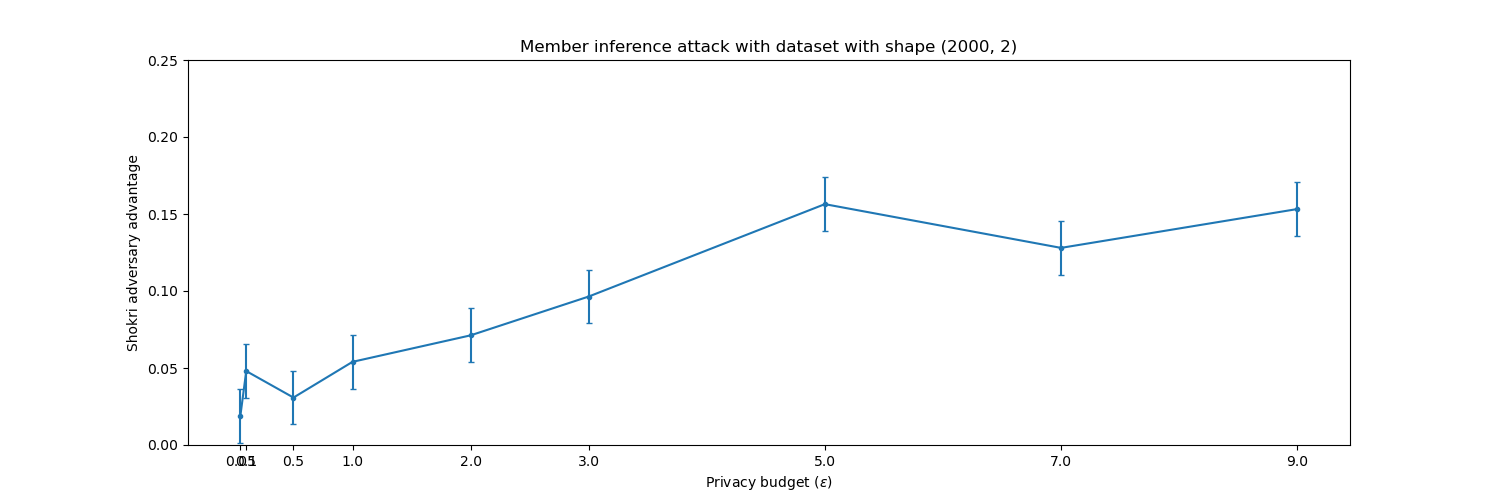
\includegraphics[width=1\linewidth]{Results/rq1/shokri_privacy_adv_2000.png}
  \caption{Shokri et al. attack mechanism using 3 shadow models and Yeom et al's adversary advantage calculated per epsilon.}
\end{figure}
\begin{figure}[!htb]
  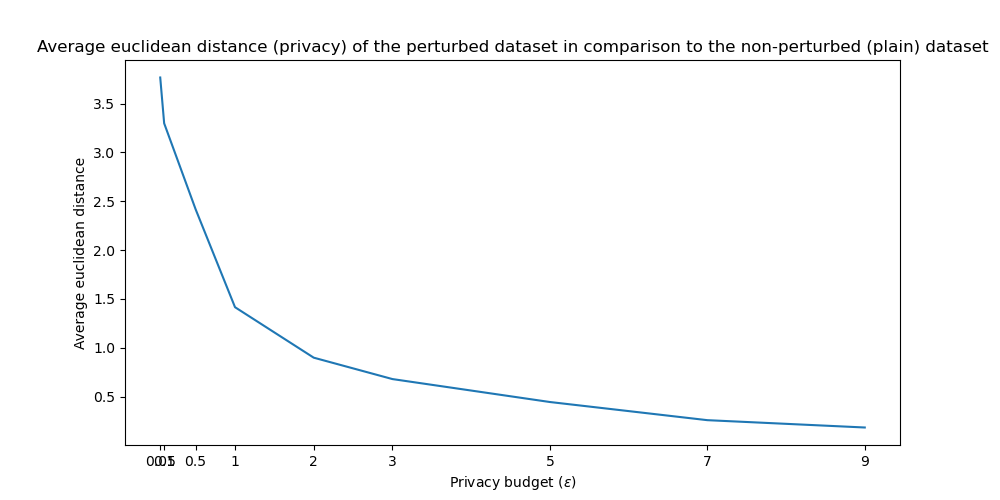
\includegraphics[width=1\linewidth]{Results/rq1/avg_euclidean.png}
  \caption{Average (euclidean) distance protection provided per epsilon.}
\end{figure}
\subsection{Research question 2}
\subsection{Research question 3}